\section{Methods}

\subsection{Semi-supervised VOS}
test
% Single Object

% \mtodo{Sort by IoU: 
% 	LucidTracker~\cite{LucidTracker}, 
% 	OnAVOS~\cite{OnAVOS},
% 	OSVOS$^\text{S}$~\cite{OSVOS-S}, 
% 	SGV~\cite{SGV},
% 	MaskRNN~\cite{MaskRNN},
% 	OSVOS~\cite{OSVOS}, 
% 	MSK~\cite{MSK},
% 	OSMN~\cite{OSMN}, 
% 	SFL~\cite{SFL}, 
% 	CTN~\cite{CTN}, 
% 	VPN~\cite{VPN}, 
% 	PLM~\cite{PLM}, 
% 	OFL~\cite{OFL}, 
% 	BVS~\cite{BVS}, 
% 	FCP~\cite{FCP}, 
% 	JMP~\cite{JMP}, 
% 	HVS~\cite{HVS}, 
% 	SEA~\cite{SEA} 
% }


% Mutliple Objects


% \mtodo{Sort by IoU: 
% 	DyeNet~\cite{DyeNet}, 
% 	MaskRNN~\cite{MaskRNN}, 
% 	OSVOS~\cite{OSVOS}, 
% 	OSMN~\cite{OSMN}, 
% 	LucidTracker~\cite{LucidTracker},
% 	OSVOS$^\text{S}$~\cite{OSVOS-S},
% 	MSK~\cite{MSK},
% }

\subsection{Unsupervised VOS}
Video object segmentation is the task of extracting spatio-temporal regions that correspond to object moving in at
least one frame in the video sequence. In contrast to semi-supervised VOS, unsupervised video object segmentation have 
more challages and is more practical in real world. In real world case, with the limitation of resources and the diversity of scenario,
it is difficult to simulate various outdoor scenario and collect dataset from it in laboratory. So unsupervised video object 
segmentation have more important impact on our real daily life. To better understand to unsupervised setting, here we list some
obvious difference between semi-supervised video segmentation.
\begin{enumerate}
    \item no first frame groundtruth is provided in test phase.
    \item no finetune process in test phase is needed.
\end{enumerate}

In unsupervised VOS tasks, we can regard them as zero-shot video objects segmentation. Because we cannot have any objects priors
in test phase, namely that the objects in testset does not exit in training phase. The task's main challages is that we need to infer
the primary objects which are moving in video frames automatically. The algorithm can discovers the most salient, or primary, objects,
that move against a video's background or display different color statistics. To better capture the moving objects against the background,
the object motion is the critical cue for identify salients objects throught entire video sequences. Next, we will introduce some important
methods which is commonly used in unsupervised VOS.

\subsubsection{Motion in Video Sequences}
In traditional static image semantic segmentation, the apperance information play an import role, which means that 
the performance is enough good if we can extract more reliable apperance features. But in video setting, thera are various
difficult challlenges caused by object moving, which are motion blur and ambigious and occluated. We just rely on apperance information
, which can  fail in this specifical scenario. Motion information can greatly help reduce this ambigious. We can capture more temporal information
to help locate objects in videos frames.

Jain $et.al$ \cite{Jain2017FusionSeg} propose an end-to-end learning framework for segmenting generic objects in video,
which learns to combine appearance and motion information to produce pixel level segmentation masks for all prominent objects.
They design a two-stream fully convolutional neural network which fuses together motion and apperance in a unified framework.
\begin{figure}[ht]
    \centering
    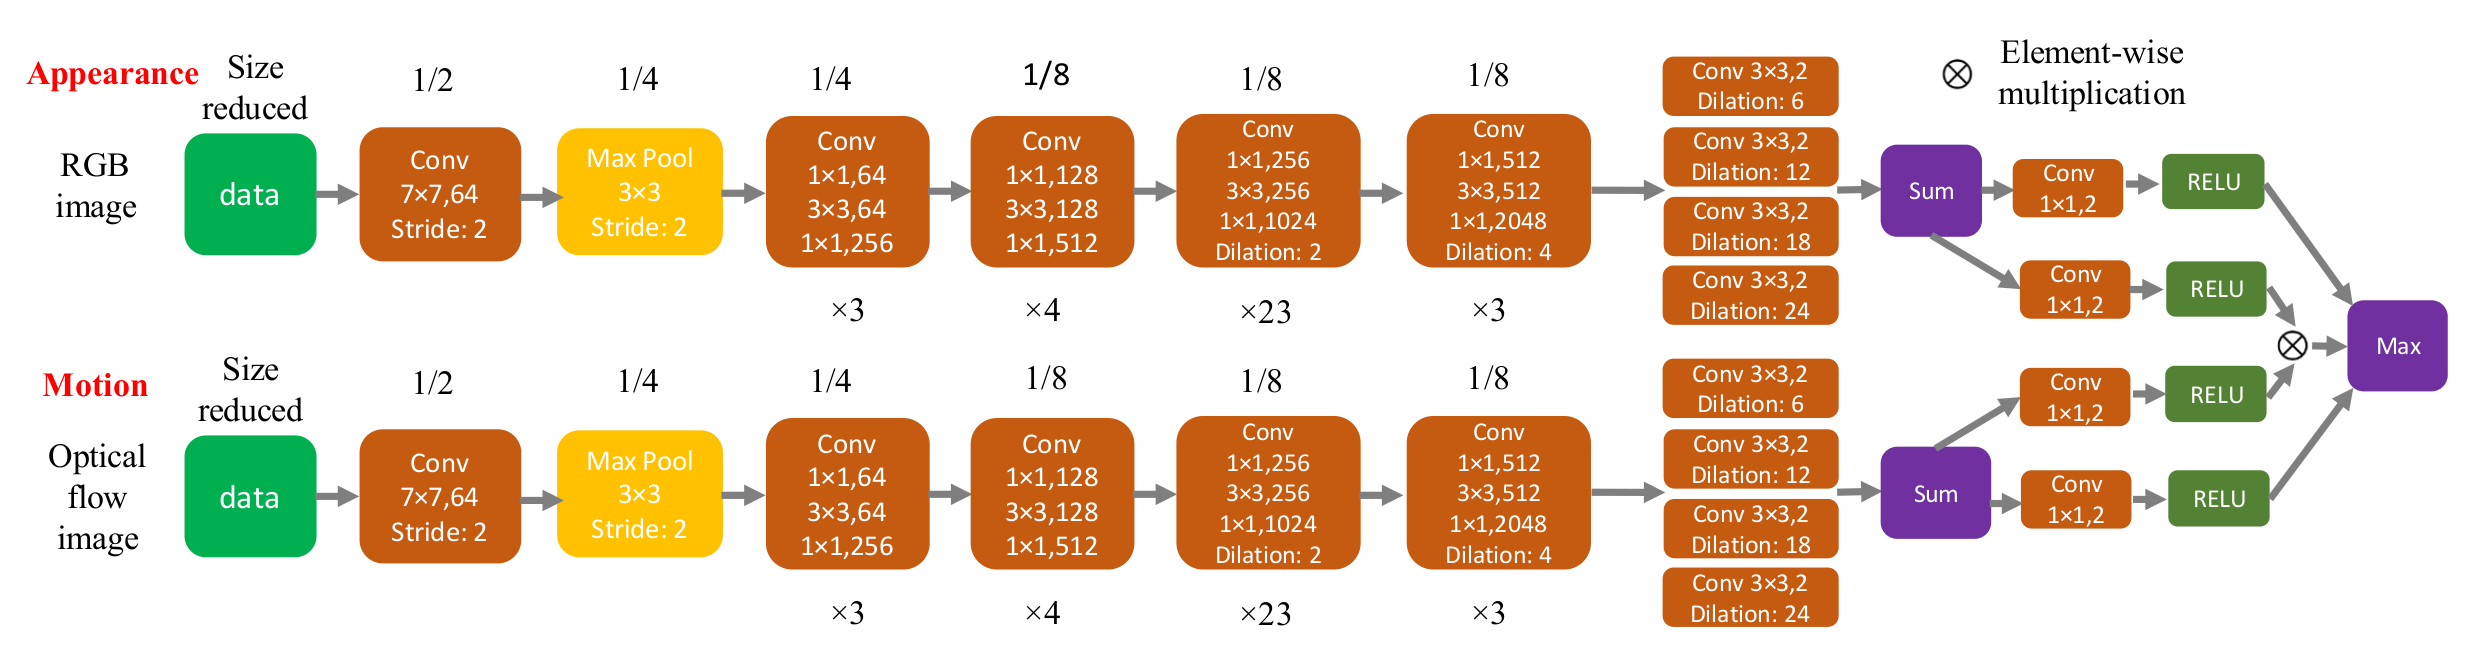
\includegraphics[width=0.5\textwidth]{./figure/FSEG_NET.png}
    \caption{FSEG Network}
    \label{FSEG}
\end{figure}

As shown in Fig \ref{FSEG}, the network can take two different inputs, which are raw images and optical flow images respectively.
The motion branch can map the motion into foreground objects, which can greatly capture temporal infomation.
In the last fusion stage, this method does not simply concat two stream feature to get the final prediction.
They design a new fusion strategy to create three independent parallel branches. They apply $1\times1$ convolution to apperance and
motion branch. Finally they apply a layer that thkes the elements-wise maximum to obtain the final prediction. The movivation is that 
an object segmentation prediction is reliable if 1) either apperance or motion model along predicts the object 
segmentation with very strong confidence or 2) their combination together predicts the segmentation with high confidence. 

Besides the two stream strategy, 




% \mtodo{Sort by IoU:
% 	% IET~\cite{li2018instance}, 
% 	ARP~\cite{koh2017}, 
% 	LVO~\cite{tokmakov17}, 
% 	FSEG~\cite{jain2017}, 
% 	LMP~\cite{tokmakov2017}, 
% 	SFL~\cite{cheng2017sfl}, 
% 	FST~\cite{papazoglou2013}, 
% 	CUT~\cite{keuper2015}, 
% 	NLC~\cite{faktor2014}, 
% 	MSG~\cite{ochs2011}, 
% 	KEY~\cite{lee2011}, 
% 	CVOS~\cite{taylor2015},
% 	TRC~\cite{fragkiadaki2012}
% }
